\section{Einleitung}

\subsection{Automatic Music Transcription}
Musik ist seit Jahrtausenden ein zentraler Bestandteil unserer Gesellschaft.
Während etwa 2000 bis 0 v.Chr. musikalische Werke meist mündlich überliefert wurden,
entwickelte sich in diesem Zeitraum auch eine Notenschrift.
Diese Notenschrift ermöglichte es, Musikstücke einfacher zu erlernen und einem breiteren Publikum zugänglich zu machen.
Durch die Digitalisierung erhielten Digital Audio Workstations zunehmend Einzug in die Musikproduktion,
wodurch Notenblätter oft nicht mehr notwendig waren und es weniger Bedarf gab diese Lieder zu übersetzen in Notenschrift.

An dieser Stelle setzt Automatic Music Transcription (AMT) an.
AMT ist ein Prozess, bei dem eine Audiospur als Input gegeben wird und diese durch Computerprogramme
Notenblätter oder, was weiter verbreitet ist, MIDI-Dateien als Output wiedergeben.
Dabei werden durch mehrere Prozesse die Eigenschaften der Noten, zum Beispiel Frequenz oder Lautstärke,
analysiert und im Kontext des Musikstückes analysiert.

\subsection{Herausforderungen und Hindernisse}
Anstatt das man selber diese Lieder, alleine durchs Gehör,
in Notenschrift überträgt würde diese Aufgabe eine Software für einen erledigen.
Dieses Ziel ist jedoch schwer zu erreichen,
da Musik mehrdimensional ist durch zum Beispiel Zeit, Tonhöhe und Polyphonie.
Vor allem bei polyphonen Musikstücken haben herkömmliche Algorithmen häufig Schwierigkeiten.
In diesen Fällen müssen sie nämlich mehrere verschiedene Stimmen gleichzeitig analysieren und
im späteren auch die jeweiligen Töne voneinander differenzieren und eindeutig einem Instrument zuordnen.
Ein weiteres Problem ist die Individualität jedes Musikstückes.
In realen Aufnahmen können leichtes Rauschen,
kleine Spielfehler oder stilistische Mittel wie Vibrato auftreten,
die je nach Interpreten unterschiedlich klingen.
Zudem sind die meisten AMT-Modelle auf westliche Tonleiter trainiert.
Dies kann zu Problemen führen, wenn man zum Beispiel
arabische oder indische Musikstücke transkribieren möchte.

\subsection{AMT und Künstliche Intelligenz,}
Um diese Vielfalt zu bewältigen, ist ein neuer, oft genutzter Ansatz,
die Nutzung von künstlicher Intelligenz und Machine Learning.
Im Gegensatz zu Algorithmen ist KI flexibler und kann sich besser
einstellen auf kleine Abweichungen in Musikstücken.
Reale Audiospuren besitzen immer eine gewisse Menge Rauschen.
Das kann bei der automatischen Musiktranskription für schwierigkeiten sorgen,
da Algorithmen diese als zusätzliche Noten ansehen oder richtige Noten dadurch nicht erkennen könnten.
KIs können sich besser an diese begebenheiten anpassen,
da neuronale Netzwerke mit genau diesen unperfekten Audiosignalen trainiert werden können.
Somit können AMT-Systeme besser angepasst werden für einen realistischen Gebrauch.

Auch die Mehrdimensionalität von Musik kann KI deutlich besser bewältigen als Algorithmen.
Neuronale Netze besitzen eine mehrdimensionale Struktur, die es ihnen ermöglicht,
verschiedene Muster, Stimmen und Eigenschaften zu erlernen.
\cite{graves2007multi}
Auf der anderen Seite müssen klassische Algorithmen diese verschiedenen Dimensionen
explizit modellieren und sind nicht in der Lage, Muster selbstständig zu erkennen.
Sie folgen nur dem, was zuvor vom Menschen fest einprogrammiert wurde.

In der automatischen Musiktranskription nutzt man meistens Spektrogramme, zur darstellung der Audiodatei.
Spektrogramme zeigen den zeitlichen Verlauf des Freqeunzspektrums eines Audiosignals.
Es gibt verschiedene Arten von Spektrogrammen.
Zwei Spektrogrammtypen, die häufig genutzt werden, sind CQT-Spektrogramme und Log-Mel-Spektrogramme.
CQT steht für Constant-Q Transform und in diesem Spektrogramm werden die Frequenzachsen logarithmisch aufgelöst.
Zudem bleibt der Q-Faktor konstant, dieser beschreibt das Verhältnis von Frequenz zu Brandbreite.
Das Log-Mel-Spektrogramm wird zunächst mit einer Short-Time Fourier Transform (STFT) gebildet.
STFT ist eine Methode, um ein Signal als ein Frequenzspektrum darzustellen.
Anschließend wird die lineare Frequenzachse auf eine Mel-Skala projiziert.
Das menschliche Gehör kann 200--400Hz feiner als 5000--5200Hz wahrnehmen.
Die Mel-Skala sorgt dafür, das sich das Spektrogramm dieser menschlichen Hörweise anpasst.
Insgesamt ist ein CQT-Spektrogramm besser für die automatische Musiktranskription,
da dieses Töne feiner unterscheiden kann.
Jedoch werden in neueren KI-Modellen zum großteil Log-Mel-Spektrogramme genutzt,
da diese robuster sind und vor allem besser in Transformer-basierte KI-Modellen laufen.
Im folgenden
\begin{figure}[H]
    \centering
    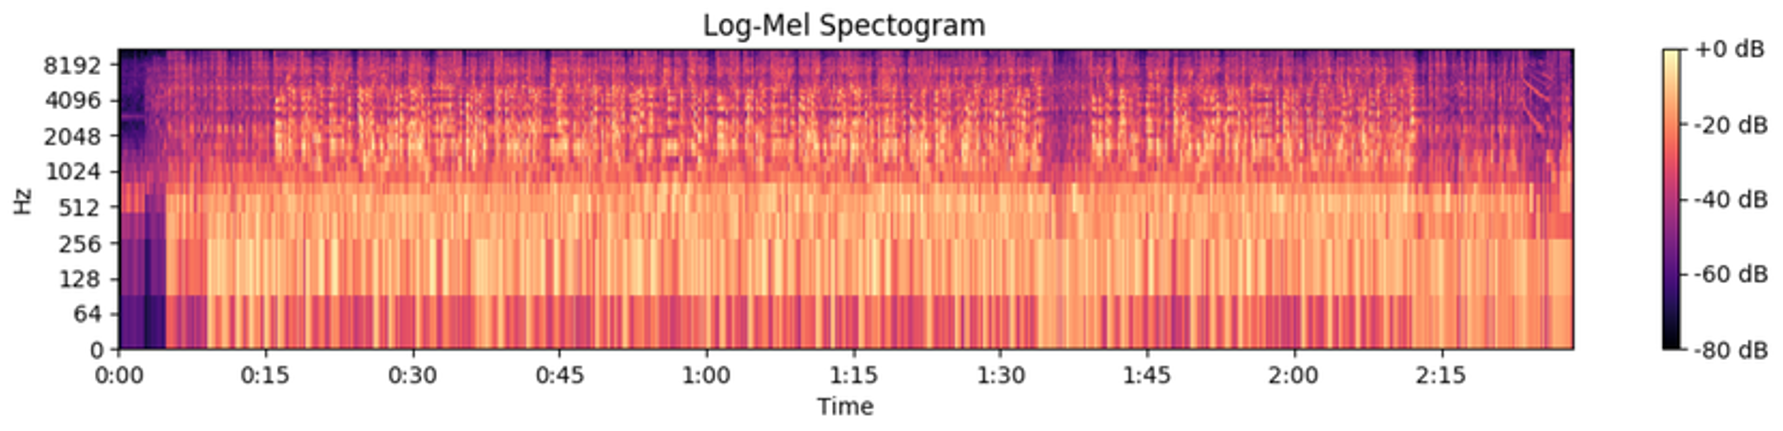
\includegraphics[width=1\textwidth]{Graphics/logMelSpek}
    \caption{Modifizierter Ausschnitt aus \cite{pyrovolakis2022multimodal}}
    \label{fig:mel-vs-logmel-mfcc}
\end{figure}

Um ein AMT-Modell mit KI zu kreieren, muss man sich auch für ein KI-Modell entscheiden.
Hier werden größtenteils Recurrent Neural Networks (RNN) oder Convolutional Neural Networks (CNN),
als einzelne Module, benutzt.
\cite{Boeck2012}
Diese Module bilden keine eigenständigen Systeme, sondern lassen sich flexibel innerhalb eines Systems kombinieren.
Da es keine objektiv richtigen oder falschen Notenfolgen gibt, ist der Einsatz von Reinforcement Learning nicht sinnvoll.
Dementsprechend braucht man auch ein zuverlässiges Datenset aus Audiodateien und deren zugehörigen MIDI-Dateien.

CNNs können gut räumliche Strukturen erkennen.
Das ist sehr hilfreich bei der Analyse von Spektrogrammen.
Meist werden die verschiedenen Frequenzen der Noten, die gespielt wurden,
nach der Verarbeitung des Musikstückes in Spektrogrammen wiedergegeben.
Durch die Analyse von dem Spektrogramm können gewisse Frequenzmuster erkannt werden,
die dann einem bestimmten Instrument zugeordnet werden können.
Das ist vor allem hilfreich dabei verschiedene Stimmen der jeweiligen Instrumente voneinander zu differenzieren.
\cite{han2016deep}

RNNs hingegen sind spezialisiert, um zeitliche Abläufe besser im Kontext zu verstehen.
In der Musik werden zahlreiche Noten hintereinander gespielt, diese müssen harmonisch im Stück übereinstimmen.
Das RNN verarbeitet die jeweiligen Sequenzen und merkt sich die Informationen der schon gespielten Noten,
um die darauffolgenden Noten besser einordnen zu können.
So lassen sich Tonfolgen harmonischen Strukturen zuordnen oder der Rhythmus des Stücks analysieren.
\cite{Boeck2012}

RNNs und CNNs werden auch häufig kombiniert in AMT-Modellen.
Meist in folgender Reihenfolge:
\begin{enumerate}
    \item \textbf{CNN:} Extrahiert folgende Merkmale aus dem Spektrogramm:
    \begin{itemize}
        \item Frequenzverteilungen und spektrale Muster
        \item Tonhöhenlage und damit verbundene Obertöne
        \item Klangfarbe einzelner Instrumente
        \item Energieverteilung, unter anderem zur Erkennung von Toneinsätzen
        \item Harmonische Strukturen wie Akkordfolgen
    \end{itemize}

    \item \textbf{RNN:} Verarbeitet auf Basis dieser Merkmale die zeitliche Abfolge und erkennt dabei folgende Eigenschaften:
    \begin{itemize}
        \item Reihenfolge und Übergänge musikalischer Ereignisse
        \item Beginn und Ende einzelner Töne zur Bestimmung der Notendauer
        \item Rhythmische Muster und zeitliche Gruppierungen
        \item Musikalische Phrasen mit zusammenhängender Struktur
        \item Wiederholungen, Themen oder längere Abhängigkeiten im Verlauf
    \end{itemize}

    \item \textbf{Output:} Gibt das transkribierte Musikstück in strukturierter Form aus:
    \begin{itemize}
        \item Als MIDI-Datei mit exakten Noteninformationen
    \end{itemize}
\end{enumerate}
Nachdem man die KI diesen Prozess durchlaufen lassen hat, kann man mit einem eigenen oder externen Programm
diese MIDI-Dateien zu standardisierter Notenschrift transkribieren.

Es gibt aber auch Projekte, wo nur ein bestimmter Teil dieser Kette mit KI-Modulen realisiert wird,
oder andere KI-Module verwendet werden.
Mehr zu diesen Modulen und CNNs und RNNs im Detail werden in dem Abschnitt-\ref{subsec:ki_integration} erläutert.

\subsection{praktische Anwendungsfelder und Vorteile von AMT}
AMT kann auch häufig bei anderen Problemen helfen
oder in zahlreichen Bereichen Quality-of-Life-Changes bringen.
Zum einen kann der Musikunterricht spannender und interaktiver gestaltet werden.
Es gibt eine breitere Auswahl von Musikstücken, die man den Schülern anbieten kann,
wodurch diese durch individuell angepasste Musikstücke mehr Spaß und Ehrgeiz beim lernen haben könnten.
Zudem kann man die gespielten Musikstücke der Schüler direkt beim Spielen transkribieren und gezielt erkennen,
wo der jeweilige Schüler noch Verbesserungsmöglichkeiten hat.
Grundsätzlich können deutlich mehr Musikstücke transkribiert werden,
wodurch sich große Archive aufbauen lassen.
Ein größeres Interesse an Musik wird geweckt, da Musikstücke von beliebten Serien, Filmen oder Spielen
leichter für deren Musikbegeisterte Zielgruppe zugänglich sind.
Alleine dadurch, dass Computerprogramme Musikstücke besser verstehen,
können darauf aufbauend weitere Tools für die Musikproduktion entwickelt werden.
Auch KI würde davon stark profitieren.
KI-generierte Musik würde verbessert werden, da die KI selber ein besseres Verständnis der Musik entwickelt.
Audiobasierte Suchmaschinen könnten gewünschte Musikstücke oder bestimmte Videos präziser finden.
Musik könnte barrierefreier gestaltet werden,
indem gehörlose Menschen sie lesen können und Musiker beim Spielen direktes Feedback erhalten,
ob sie die Noten korrekt gespielt haben.


\subsection{Motivation und Zielsetzung dieser Arbeit} (Noch nicht angefangen!)
Was wird in der Arbeit behandelt, worauf liegt der Fokus (z.B. KI-Methoden für AMT), warum ist das Thema relevant (z.B. für Musiker, KI-Forschung, Musikpädagogik)?

